%----------------------------------------------------------------------------------------
%	PACKAGES AND THEMES
%----------------------------------------------------------------------------------------
\documentclass[aspectratio=169,xcolor=dvipsnames]{beamer}
\usetheme{SimplePlusAIC}

\usepackage{hyperref}
\usepackage{graphicx} % Allows including images
\usepackage{booktabs} % Allows the use of \toprule, \midrule and  \bottomrule in tables
\usepackage{svg} %allows using svg figures
\usepackage{tikz}
\usepackage{makecell}
\usepackage{bbm}
\newcommand*{\defeq}{\stackrel{\text{def}}{=}}


\makeatletter
\usepackage{tikz}
\usetikzlibrary{calc}
\newcommand*\circled[1]{\tikz[baseline=(char.base)]{
    \node[shape=circle, draw, inner sep=1pt, 
        minimum height={\f@size*1.6},] (char) {\vphantom{WAH1g}#1};}}
\makeatother

%Select the Epilogue font (requires luaLatex or XeLaTex compilers)
\usepackage{fontspec}
\setsansfont{Epilogue}[
    Path=./epilogueFont/,
    Scale=0.9,
    Extension = .ttf,
    UprightFont=*-Regular,
    BoldFont=*-Bold,
    ItalicFont=*-Italic,
    BoldItalicFont=*-BoldItalic
    ]

%----------------------------------------------------------------------------------------
%	TITLE PAGE
%----------------------------------------------------------------------------------------

\title[FaCoRNet]{Kinship Representation Learning with Face Componential Relation} % The short title appears at the bottom of every slide, the full title is only on the title page
%\subtitle{Subtitle}

\author[Barbosa, Warley .V]{Warley Vital Barbosa}
%\institute[FEE CTU]{Artificial Intelligence Center \newline Faculty of Electrical Engineering\newline Czech Technical University in Prague}
% Your institution as it will appear on the bottom of every slide, maybe shorthand to save space

\AtBeginSection[]
{
  \begin{frame}{Overview}
  \tableofcontents[
    currentsection,
    sectionstyle=show/hide,
    subsectionstyle=show/show/hide
  ]
  \end{frame}
}

\date{\today} % Date, can be changed to a custom date
%----------------------------------------------------------------------------------------
%	PRESENTATION SLIDES
%----------------------------------------------------------------------------------------

\begin{document}

\begin{frame}[plain]
    % Print the title page as the first slide
    \titlepage
\end{frame}

\begin{frame}{Overview}
    % Throughout your presentation, if you choose to use \section{} and \subsection{} commands, these will automatically be printed on this slide as an overview of your presentation
    \tableofcontents
\end{frame}

%------------------------------------------------
\section{Introduction}
%------------------------------------------------

\begin{frame}{Introduction}
    \begin{itemize} 
        \item \textbf{Kinship Recognition} aims to determine whether a pair of face images has a \textbf{kinship relation}.
            \begin{itemize}
                \item It is inspired by the \textbf{biological discovery} that the appearance of a human face implies \textbf{clues about kinship-related information}.
                \item It can be \textbf{widely used} in various scenarios: finding missing children, child adoption, and social media applications.
            \end{itemize}
            \item \textbf{Facial Kinship Recognition} includes face representation learning and face similarity matching.
            \item The \textbf{main challenges} of kinship are mixed variations due to an uncontrolled environment.
                \begin{itemize}
                    \item Large gap in age;
                    \item Expression;
                    \item Pose;
                    \item Illumination, etc.
                \end{itemize}
    \end{itemize}
\end{frame}

\begin{frame}{Problem}
    \begin{itemize}
        \item Recently, the supervised contrastive approach (R40) achieved \textbf{state-of-the-art performance in Kinship Recognition}.
        \item Most existing approaches have several \textbf{issues}:
            \begin{itemize}
                \item Most methods directly exploit feature vector representations, \textbf{ignoring spatial correlation within face images}.
                \item Other approaches rely on \textbf{heuristic designs} (e.g. feature fusion approaches).
            \end{itemize}
        \item To address these issues, it is important to ask: \textit{How do humans recognize kinship relationships?}
            \begin{itemize}
                \item Humans usually first compare several biological \textbf{face components} of two people (e.g., eye color).
                \item Further \textbf{relation analysis} is carried out between these comparisons (e.g., nose similarity).
            \end{itemize}
    \end{itemize}
\end{frame}

\begin{frame}{Proposal}
    \begin{columns}[T] % Align columns at the top
        \begin{column}{0.6\textwidth} % Adjust the width to fit your content
            \begin{itemize}
                \item This work focuses on \textbf{exploiting the face components} to learn the relation between images in a pair. % clue from face components can infer the genetic relationships between them.
                    %\begin{itemize}
                    %    \item It aims to learn discriminative feature representations embedded with face component information, without a strong reliance on heuristic designs.
                    %\end{itemize}
                \item The whole architecture is named \textit{\textbf{F}ace \textbf{Co}mponential \textbf{R}elation \textbf{Net}work (\textbf{FaCoRNet})}.
                    \begin{itemize}
                        \item A \textit{Face Componential Relation (FaCoR)} module: it learns feature representations with the cross-relation between face components.
                        \item A novel \textit{Relation-Guided Contrastive Loss (Rel-Guide}: it is based on cross-attention estimation instead of heuristic tuning.
                            %\item The attention map can control the degree of penalty in the loss function. % which can let the feature representation of kin relation get closer in the feature space.
                            % \item In other words, it penalizes hard samples to learn more discriminative features.
                    \end{itemize}
            \end{itemize}
        \end{column}
        \begin{column}{0.4\textwidth}
            \begin{figure}
                \centering
                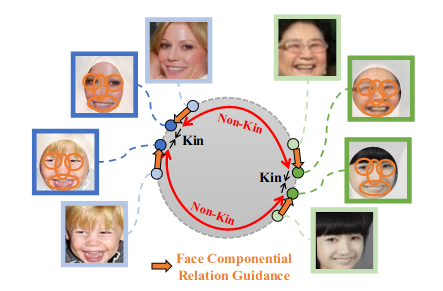
\includegraphics[width=0.9\textwidth]{imgs/F1.png}
                \caption{From the authors. Overview of the proposed relation guidance. Face components are used as clues and guide the training with the relation of facial image pairs. They claim it improves the efficacy of contrastive learning from the original whole-face features.}
                \label{fig:kfc-model-overview}
            \end{figure}
        \end{column}
    \end{columns}
\end{frame}

\begin{frame}{Contributions}
    \begin{itemize}
        \item A novel architecture called \textit{\textbf{F}ace \textbf{Co}mponential \textbf{R}elation \textbf{Net}work (\textbf{FaCoRNet})} that learns relevance from the face components with cross-attention, and adaptively learns important face components for kinship recognition.
        % This adaptability comes from the Rel-Guide, which automatically tunes the temperature based on the cross-attention map.
        \item A novel \textit{Relation-Guide Contrastive Loss} that embeds cross-relation estimates to guide the contrastive loss.
        \item The experimental results show that their proposal achieves \textbf{SOTA performance} on the largest public kinship recognition benchmark, FIW.
            %\begin{itemize}
            %    \item They also claim SOTA on KinFaceW-I and KinFaceW-II*, but that's not true.
            %\end{itemize}
    \end{itemize}
    
\end{frame}

%------------------------------------------------
\section{Related Work}
%------------------------------------------------

\begin{frame}{Kinship Recognition}
    \begin{itemize}
        \item \textbf{Traditional approaches} include designing hand-crafted feature extractors and metric learning for solving similarity metrics in kinship recognition.
        \pause
        \item Recently, \textbf{deep learning} methods have made significant advances, including two main categories:
        \pause
            \begin{itemize}
                \item \textbf{Feature Fusion}
                \item \textbf{Deep Metric Learning}
            \end{itemize}
        % Above methods have issues; proposed method tries to solve it by learning face componential correlation via cross-attention.
    \end{itemize}
\end{frame}


\begin{frame}{Kinship Recognition}
    \begin{itemize}
        \item \textbf{Feature Fusion}
            \begin{itemize}
                \item \cite{R38} utilizes the \textbf{multiple face regions} as the model inputs to learn richer facial features.
                \item \cite{R5} presents a \textbf{multi-task approach} that jointly classifies seven kinship types.
                \item \cite{R36} designs three different \textbf{feature fusion schemes} followed by direct concatenation.
                \item \cite{R29} proposes an advanced \textbf{knowledge-based tensor similarity extraction framework}.
            \end{itemize}
        \pause
        \item \textbf{Deep Metric Learning}
            \begin{itemize}
                \item \cite{R11} adopts a \textbf{fine-tuning approach} to better capture kinship features.
                \item \cite{R40} utilizes \textbf{supervised contrastive loss} -- SOTA 2021.
                \item \cite{R15} presents a \textbf{cross-pair metric learning} method that introduces a k-tuplet loss.
            \end{itemize}
        \end{itemize}
    % Above methods have issues; proposed method tries to solve it by learning face componential correlation via cross-attention.
\end{frame}

%------------------------------------------------
\section{Proposed Methods}
%------------------------------------------------

\begin{frame}{Overview}
\begin{figure}
    \centering
    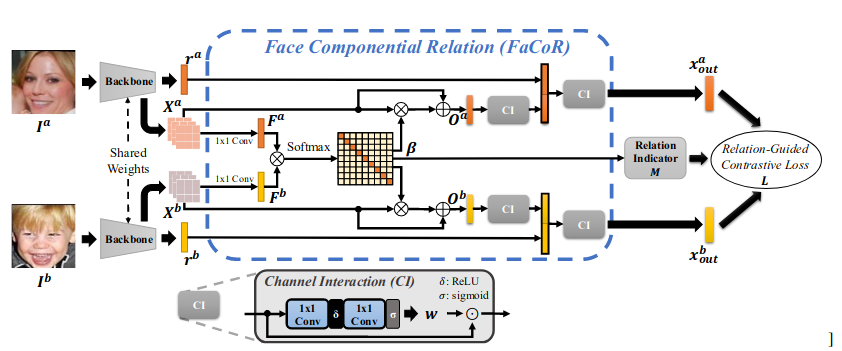
\includegraphics[width=0.75\textwidth]{imgs/F2.png}
        \caption{From the authors. Overview of the proposed \textit{Face Componential Relation Network (FaCoRNet)}. It consists of a backbone and the Face Componential Relation (FaCoR) module, trained with the Relation-Guided Contrastivee Loss \textit{L}. The cross-attention features $\mathbf{O}$ are embedded with face componential relation and fused them with the high-level features $\mathbf{r}$ via Channel Interaction (CI) blocks. During training, the attention map $\mathbf{\beta}$ is adopted as the guidance to learn discriminative representations.}
        \label{fig:model-overview}
    \end{figure}
\end{frame}

%------------------------------------------------

\begin{frame}{Face Componential Relation}
    \begin{itemize}
        \item \textit{How to properly extract and compute the relation between face components in a face image pair?}
            \begin{itemize}
                \item Most methods are \textbf{not designed for the face components} of kinship recognition.
                \item To solve this, they propose the \textit{Face Componential Relation (FaCoR)} module.
            \end{itemize}
        \pause
        \item The proposed FaCoR module mainly serves two purposes:
        \pause
            \begin{itemize}
                \item To \textbf{adaptively learn} the correlation between face image pairs, and
                \item To \textbf{learn the dependencies} in face components between image pairs.
            \end{itemize}
    \end{itemize} 
    \pause
    \begin{block}{In other words...}
        \tiny
        \[ (x_{out}^a, x_{out}^b) = (CI(CI(O^a) \parallel r^a), CI(CI(O^b) \parallel r^b)), \]
        \[ (O^a_j, O^b_j) = \left( X^a + \sum_{i=1}^N \beta_{j,i} \cdot X^a_i, X^b + \sum_{i=1}^N \gamma_{j,i} \cdot X^b_i \right), \]
        \[ \beta_{j,i} = \frac{\exp(s_{ij})}{\sum_{i=1}^N \exp(s_{ij})}, \quad s_{ij} = (F^a_i)^T F^b_j, \quad \text{where} \quad F^k = \text{Conv}_{1\times1}(X^k) \] 
    \end{block}

\end{frame}

%------------------------------------------------

\begin{frame}{Relation-Guided Contrastive Learning}
    For the standard contrastive learning, given $N$ positive samples $(x_i, y_i)$,  the contrastive loss $L$ is given by
    \begin{equation}
      L = \frac{1}{2N} \sum_{i=1}^N \left( L_c(x_i, y_i) + L_c(y_i, x_i) \right)
    \end{equation}
    and $L_c(x_i, y_i)$ is defined as
    \begin{equation}
      L_c(x_i, y_i) = -\log \frac{e^{\text{sim}(x_i, y_i)/\tau}}{\sum_{j=1}^N \mathbbm{1}_{[j \neq i]} (e^{\text{sim}(x_i, x_j)/\tau} + e^{\text{sim}(x_i, y_i)/\tau})}
    \end{equation}
    where $\mathbbm{1}_{[j \neq i]} \in \{0, 1\}$ represents an indicator function that evaluates to 1 iff $j \neq i$ and $\text{sim}(x_i, y_i)$ is the cosine similarity operation between $x$ and $y$.
\end{frame}

%------------------------------------------------

\begin{frame}{Relation-Guided Contrastive Learning}
    \begin{itemize}
        \item \textbf{Problem}: the kinship recognition performance of contrastive learning is \textbf{sensitive to hyper-parameter} $\tau$.
        \item \textbf{Solution}: \textit{Relation-Guided Contrastive Loss (Rel-Guide)} with a relation indicator $\mathbf{M}$, which \textbf{guides the contrastive loss} with the cross-attention estimation.
        \item \textbf{Main idea}: a smaller value from the cross-attention map needs a greater degree of \textbf{penalty for hard samples}.
    \end{itemize}
\end{frame}

%------------------------------------------------

\begin{frame}{Relation-Guided Contrastive Learning}
    The cross-attention map and the relation indication function are combined to enable the similarity value $\psi$ to be adaptative*
    \pause
    \begin{equation}
      L_c(x_i, y_i) = -\log \frac{e^{\text{sim}(x_i, y_i)/\psi}}{\sum_{j=1}^N \mathbbm{1}_{[j \neq i]} (e^{\text{sim}(x_i, x_j)/\psi} + e^{\text{sim}(x_i, y_i)/\psi})}
    \end{equation}
    \pause
    where $\psi = \mathbf{M}(\mathbf{\beta})/s$, $s$ is the scale value, and $\mathbf{M}$ is the global sum pooling operation.
\end{frame}


%------------------------------------------------
\section{Experiments}
%------------------------------------------------

\begin{frame}{Datasets and Evaluation}
    \begin{itemize}
        \item The compared methods are trained and tested on three publicly available kinship recognition datasets:
            \begin{itemize}
                \item Families in the Wild (FIW)
                    \begin{itemize}
                        \item In this work, they focus on the first 7 kinship relationships -- no grandparent-grandchild categories;
                        \item For evaluation, they adopt cosine similarity and thresholding to calculate accuracy;
                    \end{itemize}
                \item KinFaceW-I and II
                    \begin{itemize}
                        \item It includes only four kin relationships:  father-son (fs), father-daughter (fd), mother-son (ms), and mother-daughter (md).
                        \item For evaluation, they adopt the five-fold cross-validation in the experiments.
                    \end{itemize}
            \end{itemize}
    \end{itemize}
\end{frame}

%------------------------------------------------

\begin{frame}{Implementation Details}
    \begin{itemize}
        \item They compare \textbf{FaCoRNet} against several existing methods by using ArcFace.
        \item They also use AdaFace to demonstrate their \textbf{advanced face feature representation}.
            \begin{itemize}
                \item As the naive pre-trained weights are not suitable for the kinship method, they \textbf{modified} the hyper-parameters.
                    \begin{itemize}
                        \item Initialization as a normal distribution in range [-0.05, 0.05];
                        \item L2-norm feature normalization;
                        \item SGD as optimizer with constant lr of 1e-4 and momentum of 0.9;
                        \item Batch size = 50;
                        \item Epochs = 50.
                        \item $s = 500$ for stable training*.
                    \end{itemize}
            \end{itemize}
    \end{itemize}
\end{frame}

%------------------------------------------------

\begin{frame}{Comparison to SOTA Methods - FIW Task 1}
    \begin{figure}
        \centering
        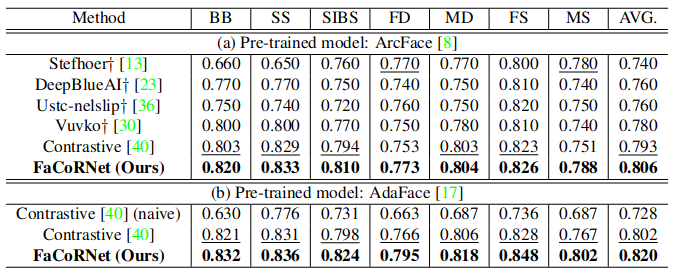
\includegraphics[width=0.75\textwidth]{imgs/T1.png}
        \caption{From the authors. The state-of-the-art performance comparison of \textit{Kinship Verification} on FIW by two pre-trained backbones: a) ArcFace and b) AdaFace. The best and second results in each column are in \textbf{bold} and \underline{underline}, respectively.}
        \label{fig:results-t1}
    \end{figure}
\end{frame}

%------------------------------------------------

\begin{frame}{Comparison to SOTA Methods - FIW Task 2}
    \begin{figure}
        \centering
        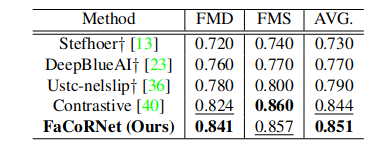
\includegraphics[width=0.5\textwidth]{imgs/T2.png}
        \caption{From the authors. The state-of-the-art performance comparison of \textit{Tri-subject Verification} on FIW. The best and second results in each column are in \textbf{bold} and \underline{underline}, respectively.}
        \label{fig:results-t2}
    \end{figure}
\end{frame}

%------------------------------------------------

\begin{frame}{Comparison to SOTA Methods - FIW Task 3}
    \begin{figure}
        \centering
        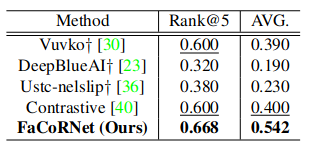
\includegraphics[width=0.5\textwidth]{imgs/T3.png}
        \caption{From the authors. The state-of-the-art performance comparison of \textit{Search and Retrieval} on FIW. The best and second results in each column are in \textbf{bold} and \underline{underline}, respectively.}
        \label{fig:results-t3}
    \end{figure}
\end{frame}

%------------------------------------------------

\begin{frame}{Comparison to SOTA Methods - KinFaceW}
    \begin{figure}
        \centering
        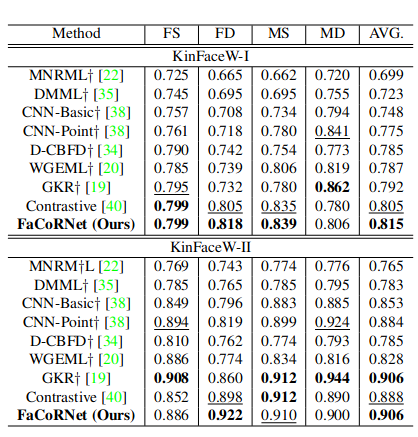
\includegraphics[width=0.4\textwidth]{imgs/T4.png}
        \caption{From the authors. Verification accuracy of different methods on KinFaceW-I and II datasets. The best and second results in each column are in \textbf{bold} and \underline{underline}, respectively.}
        \label{fig:results-t4}
    \end{figure}
\end{frame}

%------------------------------------------------

\begin{frame}{Comparison to SOTA Methods - Practical KR Protocol}
    \begin{figure}
        \centering
        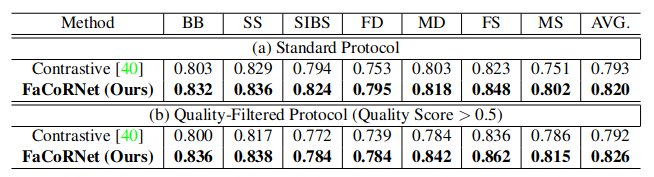
\includegraphics[width=0.75\textwidth]{imgs/T5.png}
        \caption{From the authors. Performance comparison of kinship on FIW dataset by using AdaFace to be the pre-trained model in two quality-filtered protocols: (a) standard protocol: use all image pairs without filtering; (b) quality-filtered protocol: select the image pairs with the pair quality scores larger than 0.5, which is more practical in real-world scenarios.}
        \label{fig:results-t5}
    \end{figure}
\end{frame}

%------------------------------------------------

\begin{frame}{Ablation - Component Analysis}
    \begin{figure}
        \centering
        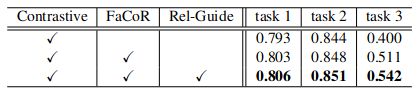
\includegraphics[width=0.5\textwidth]{imgs/T6.png}
        \caption{From the authors. Component analysis of FaCoRNet on the FIW dataset, including \textit{Kinship Verification}, \textit{Tri-subject Verification}, and \textit{Search and Retrieval} tasks, corresponding to task 1, task 2, and task 3, respectively.}
        \label{fig:results-t6}
    \end{figure}
\end{frame}

%------------------------------------------------

\begin{frame}{Ablation - t-SNE}
    \begin{figure}
        \centering
        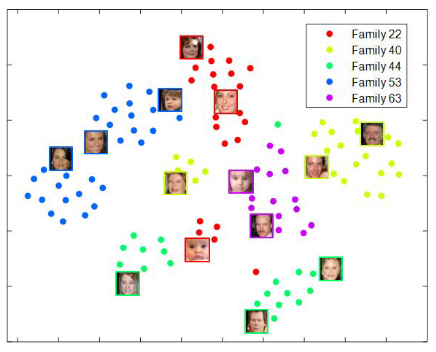
\includegraphics[width=0.5\textwidth]{imgs/F3.png}
        \caption{From the authors. Visual analysis of the learned features from 5 families from the FIW validation set with t-SNE.}
        \label{fig:results-f3}
    \end{figure}
\end{frame}

%------------------------------------------------

\begin{frame}{Ablation - Cross-Attention map}
    \begin{figure}
        \centering
        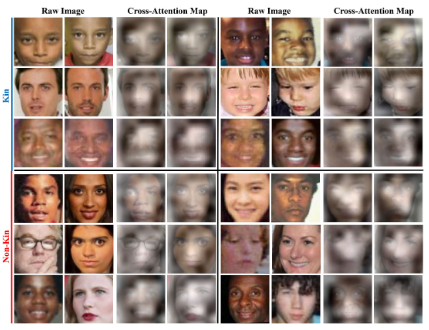
\includegraphics[width=0.5\textwidth]{imgs/F4.png}
        \caption{From the authors. Illustration of the Cross-Attention map includes kin (first to third rows) and non-kin (fourth to sixth rows) cases: the left side shows the raw image pairs and the right side shows the visualization of the cross-attention maps.}
        \label{fig:results-f4}
    \end{figure}
\end{frame}

%------------------------------------------------
\section{Conclusion and Future Work}
%------------------------------------------------
% TODO: also add my own conclusions
\begin{frame}{Conclusion}
    \begin{itemize}
        \item This work proposes a \textbf{novel} architecture named \textit{\textbf{F}ace \textbf{Co}mponential \textbf{R}elation \textbf{Net}work (\textbf{FaCoRNet})} for kinship recognition.
            \begin{itemize}
                \item An \textbf{attention-based model} designed for learning correlation between image pairs in terms of face components.
                \item \textit{Face Componential Relation (FaCoR)} module to achieve not only \textbf{adaptive learning correlation}, but also learning important face components.
                \item \textit{Relation-Guided Contrastive Loss (Rel-Guide)} that embedds the cross-attention mestimation as the \textbf{guidance to learn discriminative representations}.
            \end{itemize}
        \item Experimental results shows that this method achieves SOTA performance on multiple* kinship recognition benchmarks.
            \begin{itemize}
                \item For practical kinship recognition protocol, it also outperforms the SOTA methods by large margins.
            \end{itemize}
    \end{itemize}
\end{frame}
%------------------------------------------------

\begin{frame}{Future Work}
    \begin{itemize}
        \item The authors believe that it can be served as a \textbf{strong baseline} for further advancing facial relation learning approches.
        \item They also plan to incorporate \textbf{face quality scores} into the training process (!), aiming to mitigate the issues from low-quality face images.
        \item \textbf{Multi-modal information} (e.g., text, metadata) could also compensate the vision-based methods.
    \end{itemize}
    
\end{frame}


%------------------------------------------------
\section{Potential Directions}
%------------------------------------------------

\begin{frame}{Potential Directions}
    \begin{itemize}
        \item \textbf{Multi-level representations} (e.g., SwinFace subnetworks) from Face Recognition;
        \item \textbf{Recognizability Index} from Very Low-Resolution Face Recognition;
        \item Relation networks for \textbf{nonlinear similarity mappings} between feature representations;
        \item Face componential \textbf{relations} (as this work);
        \item Debias and von Mises...
        \item ...
    \end{itemize}
\end{frame}

\begin{frame}{References}
    % Beamer does not support BibTeX so references must be inserted manually as below
    \footnotesize{
        \begin{thebibliography}{99}

            \bibitem[Zhang et al., 2015]{R38} Zhang, K., Huang, Y., Song, C., Wu, H., Wang, L., \& Statistical Machine Intelligence. (2015)
            \newblock Kinship verification with deep convolutional neural networks
            \newblock In: The British Machine Vision Conference. BMVA Press.
            
            \bibitem[Dahan \& Keller, 2020]{R5} Dahan, E., \& Keller, Y. (2020)
            \newblock A unified approach to kinship verification
            \newblock IEEE Transactions on Pattern Analysis and Machine Intelligence, 43(8), 2851–2857.
            
            \bibitem[Yu et al., 2022]{R36} Yu, J., Li, M., Hao, X., \& Xie, G. (2022)
            \newblock Deep fusion siamese network for automatic kinship verification
            \newblock In: 2020 15th IEEE International Conference on Automatic Face and Gesture Recognition (FG 2020). IEEE, pp. 892–899.
            
            \bibitem[Serraoui et al., 2022]{R29} Serraoui, I., Laiadi, O., Ouamane, A., Dornaika, F., \& Taleb-Ahmed, A. (2022)
            \newblock Knowledge-based tensor subspace analysis system for kinship verification
            \newblock Neural Networks, 151, 222–237.
            
        \end{thebibliography}
    }
\end{frame}
            
\begin{frame}{References}
    % Beamer does not support BibTeX so references must be inserted manually as below
    \footnotesize{
        \begin{thebibliography}{99}
            \bibitem[Duan et al., 2017]{R11} Duan, Q., Zhang, L., \& Zuo, W. (2017)
            \newblock From face recognition to kinship verification: An adaptation approach
            \newblock In: Proceedings of the IEEE International Conference on Computer Vision Workshops, pp. 1590–1598.
            
            \bibitem[Zhang et al., 2021]{R40} Zhang, X., Min, X., Zhou, X., \& Guo, G. (2021)
            \newblock Supervised contrastive learning for facial kinship recognition
            \newblock In: 2021 16th IEEE International Conference on Automatic Face and Gesture Recognition (FG 2021).
            
            \bibitem[Huang et al., 2022]{R15} Huang, S., Lin, J., Huangfu, L., Xing, Y., Hu, J., \& Zeng, D. D. (2022)
            \newblock Adaptively weighted k-tuple metric network for kinship verification
            \newblock IEEE Transactions on Cybernetics.

        \end{thebibliography}
    }
\end{frame}

%------------------------------------------------

\begin{frame}
    \Huge{\centerline{\textbf{The End}}}
\end{frame}

%----------------------------------------------------------------------------------------
\end{document}